\chapter{Rapida guida all'uso di Linux}\label{linux}
Nel corso di laurea in Fisica andrai inevitabilmente a scontrarti con Linux\footnote{Ma cos'è Linux? È un ``kernel'', il cuore di un sistema operativo. Anche Android usa Linux come kernel. Quando noi diciamo ``Linux'', sottointendiamo, invece,``GNU/Linux'', una famiglia di sistemi operativi. Di GNU/Linux esistono varie ``distribuzioni'': Debian, Ubuntu, Arch, Manjaro, ecc\ldots. Per fare un parallelo, Windows è una famiglia di sistemi operativi, Windows 10 è un sistema operativo, e Windows NT è il kernel di Windows. In queste note parlo, per semplicità, di Linux come sistema operativo: permettimi l'abuso di linguaggio. }. In primis, per questo esame, per cui è il caso di imparare sin da subito alcuni comandi base: non è piacevole brancolare nel buio!

Lo strumento più potente ed importante di questo sistema operativo è il \emph{terminale}. Cos'è? Normalmente siamo abituati ad interfacciarci con il nostro PC per via grafica: visualizziamo le cartelle, i file, i contenuti\ldots Il terminal è il computer privato di grafica! In realtà, su Linux, la grafica è un'aggiunta, ma l'intero sistema operativo esiste a prescindere da essa. \\

Apri un \emph{terminale} e cominciamo! Ah già, come? Ctrl+alt+T su Ubuntu, oppure cercalo nelle utility di sistema.
Ti apparirà una finestra vuota con in alto a sinistra un \emph{nome@altro-nome altro}. Il primo è il tuo nome utente, dopo la @ c'è il nome del computer. ``Altro'' (che non necessariamente è presente) tipicamente indica la cartella dove ti trovi(vedi \ref{filesystem}). Ci siamo: il modo per interfacciarsi al computer, privato della grafica, è scrivendo comandi (per dare un comando, scrivilo e premi invio) e ricevendo output di soli caratteri. 

Il comando base, che spesso viene ignorato, è \textbf{man}: sta per \emph{manual}. Prova a scrivere ``man man'' e, come per tutti i comandi, premere invio.  Ti apparirà la \emph{manual page} del comando scritto alla destra di ``man'' (che in questo caso è di nuovo ``man''): in poche parole il manuale del comando. Se non sai come funziona un comando o non ti ricordi come si usa, il modo più rapido ed efficace è scrivere proprio ``man comando'' e ti verrà mostrato il suo manuale. Per uscire da una \emph{man page} schiaccia ``q'' (quit). 

\section{Il filesystem}\label{filesystem}
Il filesystem, senza entrare troppo nei dettagli, è come vengono organizzati in memoria file e cartelle. 

Linux si comporta come un albero: partendo dalla \emph{radice} --\emph{``root''}--, il filesystem si dirama nelle varie cartelle --\emph{``directory''}--. Dentro ogni cartella sono contenuti i file e le cartelle successive. Una pulce nell'orecchio: su Linux tutto è un file, anche le cartelle.\\

\subsection{Navigare nel filesystem}
Se sul tuo terminale scrivi ``\textbf{ls}'' (che pressapoco significa ``list directory contents''), puoi visualizzare il contenuto della cartella in cui ti trovi.

Ogni cartella è quindi un ramo dell'albero; partendo dalla \emph{radice}, la quale è rappresentata da \textbf{/} (lo slash). 

In figura \ref{dirgraph} puoi vedere la rappresentazione grafica della \emph{radice} con le sue sottocartelle. In figura \ref{dirter}, invece, c'è l'output del terminale. Come vedi, quest'ultimo è composto dai nomi delle sottocartelle e dei file contenuti nella cartella in cui ti trovi.

\begin{figure} [ht]
	\centering
	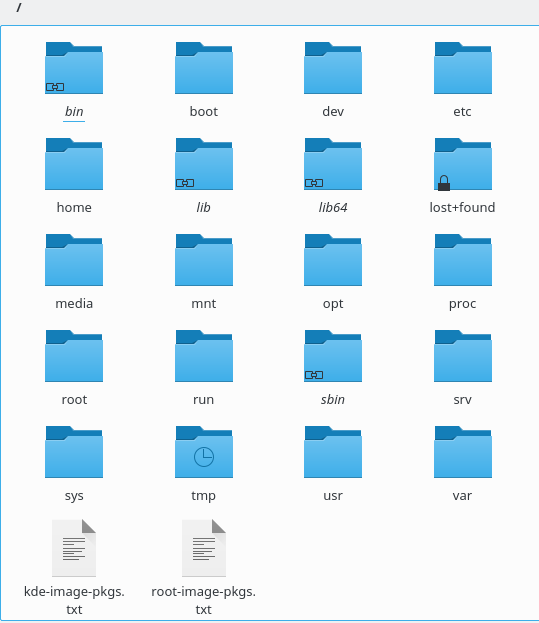
\includegraphics[scale=0.3]{Immagini/dir_graph.png}  
	\caption{}
	\label{dirgraph}
\end{figure}
\begin{figure} [ht]
	\centering
	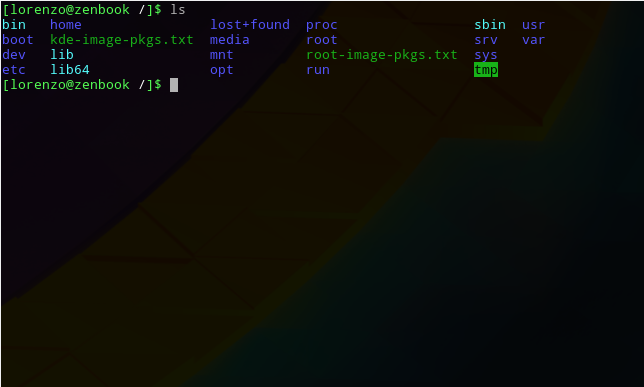
\includegraphics[scale=0.45]{Immagini/dir_ter.png}  
	\caption{}
	\label{dirter}
\end{figure}

Non ci interesseremo a cosa sono tutte queste cartelle, ce n'è solo una che ti deve importare: ``home''. Dentro vi sono le cartelle base di tutti gli utenti, la loro \emph{home}. Ogni utente può accedere solo alla propria. 

Ma come ci si sposta tra le cartelle? Il comando è \textbf{cd} (change directory), che alla sua destra vuole la cartella in cui ci vogliamo spostare. Abbiamo visto che il simbolo della \emph{radice} è lo \emph{slash}, il simbolo della tua home è invece la tilde ( \textasciitilde). I comandi \verb|cd ~| e \verb|cd /| ti faranno spostare, rispettivamente, nella mia \emph{home} e nella \emph{radice}. Se lanci ``\verb|cd|'' senza alcun argomento, ti sposterai nella tua \emph{home} (è equivalente alla tilde). \\

Bisogna subito imparare l'importantissima differenza tra \emph{percorso assoluto} e \emph{percorso relativo}. 

Poniamo di essere l'utente ``pippo'' e di avere una cartella, nella nostra \emph{home}, chiamata ``fuffa''. Se ci troviamo nella \emph{home} il comando per spostarsi in fuffa sarà \verb|cd fuffa|. Perché? Semplicemente, il percorso \emph{relativo} di questa cartella rispetto a dove ci troviamo è ``fuffa'', si trova lì! Se invece ci troviamo in un posto qualsiasi (diverso dalla \emph{home}), possiamo scrivere il percorso \emph{assoluto} di fuffa. Il comando sarà \verb|cd /home/pippo/fuffa|: i percorsi assoluti sono indicati partendo dalla \emph{radice}, e le sottocartelle si separano con degli slash. Quindi, partendo dalla \emph{radice}, a grandi linee, significa ``spostati in \emph{home} (che contiene le \emph{home} di tutti gli utenti), quindi in pippo (la \emph{home} di pippo), quindi in fuffa''. 

Chiaro? Il \emph{percorso assoluto} è espresso indicando tutte le sottocartelle a partire dalla \emph{radice}, il \emph{percorso relativo} è espresso indicando le sottocartelle a partire da dove ci troviamo. 

Spesso lavoriamo in cartelle che appartengono alla nostra \emph{home}; per abbreviare, al posto del percorso completo possiamo usare \verb| cd ~/percorso|: la tilde iniziale esprime il fatto che il percorso deve essere inteso a partire dalla nostra \emph{home}.

In Linux ci sono due cartelle particolarissime, presenti ovunque: la cartella ``punto'' (si, proprio `` . '') e la cartella ``punto punto'' (`` .. ''). La prima rappresenta la cartella stessa in cui siamo (se sono nella cartella fuffa e scrivo \verb|cd .| mi sposto nella cartella in cui sono, ovvero non mi sposto). La cartella ``..'' rappresenta quella precedente nell'albero: se sono in ``fuffa'' e scrivo \verb|cd ..| mi sposto in ``pippo'' (la cartella precedente).

Fai dunque attenzione: i comandi \verb|cd fuffa/fuffa1/fuffa2| e \verb|cd /fuffa/fuffa1/fuffa2| sono diversi! ( Questa differenza è fondamentale, e fonte di errori enormi!)

Mentre i comandi \verb|cd fuffa/fuffa1/fuffa2| e \verb|cd ./fuffa/fuffa1/fuffa2| sono uguali! Per il comando \verb|cd|, mettere o non mettere uno slash alla fine del percorso è indifferente: \verb|cd fuffa| e \verb|cd fuffa/| sono equivalenti (e volendo anche \verb|cd fuffa/.|). Complicato? Con un po' di pratica diventerà tutto ovvio. 

E se ci siamo persi? Il comando ``\textbf{pwd}'' restituisce il percorso assoluto della nostra posizione. 
\subsection{Modificare il filesystem}\label{modfile}
Ora che abbiamo visto come muoverci nel filesystem di Linux è arrivato il momento di capire come creare, rimuovere e modificare cartelle e file.

Il comando ``\textbf{mkdir} \emph{nomecartella}'' crea una cartella nell'attuale posizione con il nome alla sua destra (mkdir: make directory, facile!). È anche possibile esplicitare il percorso dove vogliamo creare la cartella: ``\verb|mkdir /home/pippo/nuovacartella|'' è un comando valido (supponendo che vogliamo creare \emph{nuovacartella} dentro la cartella \emph{pippo}).

Per creare un file vuoto il comando è ``\textbf{touch} \emph{nomefile}''. Una nota: in Linux, le estensioni non hanno alcun significato; per cui, un file di testo può essere chiamato ``file'', ``file.txt'', ``file.dat'', ``file.quellochevuoi'', ecc\ldots

Per aprire (ed eventualmente creare, se non esiste) un file con il nostro editor di testo preferito, il comando è ``editor nomefile'', per cui, ad esempio usando gedit: ``\verb|gedit file.txt|''. Il problema di un comando di questo tipo è che il terminale lancia l'editor di testo e rimane in uno stato di attesa: fino a che l'editor non viene chiuso non possiamo più agire con il terminale. Esiste un trucco: porre una ``\&'' alla fine del comando, in questo modo ci viene restituito il terminale dal programma lanciato e possiamo continuare ad utilizzarlo (nota, però, che se chiudiamo il terminale muore anche il programma). Quindi, alla fine dei conti, il comando più efficace per aprire un file con gedit è ``\verb|gedit file &|''. 

Per rimuovere un file, il comando è ``\textbf{rm} \emph{nomefile}'' (rm sta per remove). Per rimuovere una cartella dobbiamo renderlo ricorsivo, ovvero rimuovere anche tutti i contenuti della cartella; per farlo si usa ``\textbf{rm -r} \emph{nomecartella}''. ATTENTO: su Linux rm non sposta in alcun ``cestino'', elimina senza possibilità di ritorno.

Per copiare un file usiamo: ``\textbf{cp} \emph{percorso-iniziale} \emph{percorso-di-arrivo}''. Se vogliamo copiare il file nella stessa cartella allora useremo ``\verb|cp nomefile nomecopia|''. Per le cartelle bisogna copiare anche tutti i file contenuti, quindi usare cp in modo ricorsivo: ``\textbf{cp -r} \emph{percorso-cartella-da-copiare} \emph{percorso-copia}''. 


L'ultimo comando base utile è ``\textbf{mv}'' (move); mv è ambivalente, può significare sia ``rinomina'' sia ``sposta'' (ma, se ci rifletti bene, in realtà sono la stessa cosa: ``mv'' cambia il percorso nel filesystem). Se scriviamo ``\verb|mv vecchionome nuovonome|'' stiamo rinominando: se ci pensi, un indirizzo nel filesystem è del tipo /x/y/z/a/b/... Scrivendo ``vecchionome'' e ``nuovonome'' sottintendiamo che tutto quello che viene prima rimane immutato, cambia solo l'ultima parte dell'indirizzo, ovvero il nome! Per le cartelle non bisogna utilizare il ``-r'' (prova a riflettere: perché non bisogna rendere il comando ricorsivo? Perché basta cambiare l'indirizzo della cartella e non anche di tutte le cose contenute?). \\
Se scriviamo ``\verb|mv vecchio-percorso nuovo-percorso|'' stiamo spostando il file o la cartella. \\

Per tutti i comandi elencati in \ref{modfile} usare \emph{percorso assoluto} o \emph{relativo} è indifferente. 

\section{Secure Shell: Linux in remoto}
Come ti avranno detto nel corso di Informatica, puoi accedere in remoto al laboratorio di calcolo e lavorare da casa. 

Un enorme pregio di Linux è quello che si può accedere ad una \emph{shell} (un \emph{terminale}) in remoto. Esistono anche programmi per Windows che ti permettono di farlo ma, data la mia scarsissima conoscenza di quel sistema operativo, in queste note non troverai  istruzioni per farlo\ldots Chiedo venia e ti rimando al sito del corso di Informatica dove puoi cercare ``putty''.
Se invece sei un Mac-user o hai una partizione con Linux, allora è facilissimo: ``\verb|ssh nomeutente@nomeserver|''. Se ti vuoi collegare al laboratorio di calcolo, il comando sarà: ``\verb|ssh tuonomeutente@tolab.fisica.unimi.it|'' (generalmente il tuo nome utente è quello della mail di Ateneo). Se vuoi avere anche una sessione grafica (ad esempio per aprire programmi come gedit, altrimenti disponi solo del terminale) devi usare ``\verb|ssh -X|'' (X volutamente maiuscola).

Una volta entrato nel server di destinazione, è come se ti trovassi fisicamente su quel computer: il terminale è di quel computer e valgono tutti i comandi spiegati precedentemente. Quando hai finito di lavorare e desideri ritornare sul tuo computer ti basta usare il comando ``\verb|exit|''.\\

Un altro comando utile è ''\textbf{scp}'' (secure copy). Molto semplicemente, si comporta come il comando cp, tenendo conto, però, che uno dei due indirizzi è sul server di destinazione. Ecco degli esempi pratici:
\begin{itemize}
	\item Copiare un file locale su un server di destinazione:
	
	\verb|scp indirizzo_file nomeutente@nomeserver:indirizzo_destinazione|
	(nessuno spazio dopo i due punti!)
	\item Copiare un file remoto sul mio computer:
	
	\verb|scp nomeutente@nomeservr:indirizzo_file_destinazione indirizzo_su_mio_computer|
\end{itemize}

Due precisazioni: la prima è che per copiare una cartella bisogna usare il comando ricorsivo ``\verb|scp -r|''; la seconda precisazione è che gli indirizzi sul server di destinazione sono relativi alla tua \emph{home}, ovviamente puoi inserirli in maniera completa, utilizzando quelli assoluti.
